\chapter{Sending and Receiving Data}
\label{chap:encoding}%

Typically you use sockets because your program needs to provide
information to, or use information provided by, another program. There
is no magic: any programs that exchange information must agree on how
that information will be \emph{encoded}---represented as a sequence of
bits---as well as which program sends what information when, and how
the information received affects the behavior of the program.  This
agreement regarding the form and meaning of information exchanged over
a communication channel is called a \emph{protocol}; a protocol used
in implementing a particular application is an \emph{application
protocol}.  In our echo example from the earlier chapters, the
application protocol is trivial: neither the client's nor the server's
behavior is affected by the \emph{contents\/} of the messages they
exchange.  Because in most real applications the behavior of clients
and servers depend upon the information they exchange, application
protocols are usually somewhat more complicated.

The TCP/IP protocols transport bytes of user data without examining or
modifying them.  This allows applications great flexibility in how
they encode their information for transmission.  Most application
protocols are defined in terms of discrete \emph{messages} made up of
sequences of \emph{fields}.  Each field contains a specific piece of
information encoded as a sequence of bits.  The application protocol
specifies exactly how these sequences of bits are to be arranged by
the sender and interpreted, or \emph{parsed}, by the receiver so that
the latter can extract the meaning of each field.  About the only
constraint imposed by TCP/IP is that information must be sent and
received in chunks whose length in bits is a multiple of eight.  So
from now on we consider messages to be sequences of \emph{bytes}.
Given this, it may be helpful to think of a transmitted message as a
sequence or array of numbers, each between 0 and 255.  That
corresponds to the range of binary values that can be encoded in 8
bits: 00000000 for zero, 00000001 for one, 00000010 for two, and so
on, up to 11111111 for 255.

When you build a program to exchange information via sockets with
other programs, typically one of two situations applies: either you
are designing/writing the programs on both sides of the socket, in
which case you are free to define the application protocol yourself,
or you are implementing a protocol that
someone else has \emph{already\/} specified, perhaps a protocol
\emph{standard}.  In either case, the basic principles of encoding and
decoding different types of information as bytes ``on the wire'' are
the same.  (By the way, everything in this chapter also applies if the
``wire'' is a file that is written by one program and then read by
another.)

\section{Encoding Integers}
\label{sect:encodingInts}

Let's first consider the question of how integers---that is,
groups of bits that can represent whole numbers---can be
sent and received via sockets.  In a sense, all types of information are
ultimately encoded as fixed-size integers, so the ability to send and receive
them is fundamental.

\subsection{Sizes of Integers}

We have seen that TCP and UDP sockets transmit sequences of
 \emph{bytes}:
groups of 8 bits, which can contain whole number values in the range
 0--255. 
%
Sometimes it is necessary to send integers whose value might be
bigger than 255; such integers must be encoded using multiple bytes.
%
To exchange fixed-size, multi-byte integers, the sender and receiver
have to agree \emph{in advance\/} on several things.
The first is the \emph{size\/} (in bytes) of each integer to be sent.

For example, an \type{int} might be stored as a 32-bit quantity.
%
In addition to \type{int}, the C language defines several other integer
types: \type{short}, \type{char}, and \type{long}; the idea is that
these integers can be different sizes, and the programmer can use the
one that fits the application.
%
Unlike some languages, however,
the C language does \emph{not\/} specify the exact size
of each of these primitive types.  Instead, that is left up to the
implementation.  Thus, the size of a \type{short} integer can vary from
platform to platform.\footnote{By ``platform'' in this book we mean
  the combination of compiler, operating system and hardware
  architecture.  The gcc compiler with the Linux operating system,
  running on Intel's IA-32
  architecture is an example of a platform.} 
The C language specification does say that a \type{char} is no bigger than
a \type{short}, which is no bigger than an \type{int}, which is no bigger
than a \type{long}, which is no bigger than a \type{long long}.
%XXXX INCLUDE LONG LONG?
However, the specification does \emph{not\/} require that these types
actually be different sizes---it is technically possible for a
\type{char} to be the same size as a \type{long}!
On most platforms, however, the sizes do differ, and it is a safe
bet that they do on yours, too.

So how do you determine the exact size of an \type{int} (or \type{char}, or
\type{long}, or \ldots) on your platform?
The answer is simple: use the \fcnsys{sizeof( )} operator, which returns
the amount of memory (in ``bytes'') occupied by its argument (a type
or variable) on the current platform.
Here are a couple of things to note about \fcn{sizeof( )}.  First, the
language specifies that \fcn{sizeof(char)} is 1---\emph{always}.
Thus a ``byte'' is the amount of space occupied by a variable of type
\type{char}, and the units 
of \fcn{sizeof( )} are actually ``\fcn{sizeof(\type{char})}''.
But exactly how big is a byte?  That's the second thing:
the predefined constant \const{CHAR\_BIT} tells how many bits it takes
to represent a value of type \type{char}---usually eight,
but possibly 10 or even 32.

While it's always possible to write a 
simple program to print the values returned by \fcn{sizeof()} for
the various primitive integer types, and thus clear up any mystery
about integer sizes on your platform, C's lack of specificity about
the size of its primitive integer types makes it a 
little tricky if you want to write portable code for sending
integers of a specific size over the Internet.  Consider the problem
of sending a 32-bit integer over a TCP connection.  Do you use an
\type{int}, a \type{long}, or what?
On some machines an \type{int} is 32 bits,
while on others a \type{long} may be 32 bits.

The C99 standard offers a solution in the form of a set of optional types:
\type{int8\_t}, \type{int16\_t}, \type{int32\_t}, and \type{int64\_t}
(along with their unsigned counterparts \type{uint8\_t}, etc) all
have the size (in bits) indicated by their names.  On a platform where
\const{CHAR\_BIT} is eight,\footnote{%
We are not aware of any modern general-purpose computing platform
where \const{CHAR\_BIT} differs from eight.
Throughout the rest of this book, the value of
\const{CHAR\_BIT} is assumed, without comment, to be 8.}
%
these are one-, two-, four- and eight-byte integers, respectively.
%
Although these types may not be implemented on every platform,
each \emph{is\/} required to be defined if any native primitive type
has the corresponding size.  (So if, say, the size of an \type{int} on the
platform is 32 bits, the ``optional'' type \type{int32\_t} is
\emph{required\/} to be defined.)
%
Throughout the rest of this chapter, we make use of these types to
specify the precise size of the integers we want.  We will also make
use of the C99-defined type \type{long long}, which is typically
larger than a long.
%
Program \file{TestSizes.c} will print the value of \const{CHAR\_BIT},
the sizes of all the primitive integer
types, and the sizes of the
fixed-size types defined by the C99 standard.
%
%%%%%%%%%%%%%%%%%%%%%%%%%%%%%%%%%%%%%%%%%%%%%%%%%%%%%%%%%%%%%%%%
\jcode{TestSizes.c}{code/TestSizes.c}{1}{1}
%%%%%%%%%%%%%%%%%%%%%%%%%%%%%%%%%%%%%%%%%%%%%%%%%%%%%%%%%%%%%%%%
%

To make things a little more concrete, in the remainder of this section
we'll consider the problem of encoding a sequence of
integers of different sizes---specifically, of one, two, four, and
eight bytes, in that order.
Thus, we need a total of 15 bytes, as shown in the figure below.
%
\jfigs{figures/intlayout.eps}{\textwidth}
%
We'll consider several different methods of doing this, but in all
cases we'll assume that the C99 fixed-size types are supported.

\subsection{Byte Ordering}
\label{sect:byteordering}
Once the sender and receiver have specified the sizes of the integers
to be transmitted, they need to agree on some other aspects.
For integers that require more than
one byte to encode, they have to answer the question of which \emph{order\/} to
send the bytes in.

There are two obvious choices:  start at the ``right'' end
of the number, with the least significant bits---so-called
\emph{little-endian\/} order---or at the left end, with the most
significant bits---\emph{big-endian\/} order.  (Note that
the ordering of \emph{bits within bytes\/} is, fortunately,
handled by the implementation in a standard way.)
%
Consider the \type{long long} value 123456787654321L.
Its 64-bit representation (in hexadecimal) is \const{0x0000704885F926B1}.
If we transmit the bytes in big-endian order, the sequence of
(decimal) byte values will look like this:
% XXX LINE BREAK HERE
\jfigs{figures/bigendianlong.eps}{0.6\textwidth}
%
If we transmit them in little-endian order, the sequence will be:
% XXX LINE BREAK HERE
\jfigs{figures/littleendianlong.eps}{0.6\textwidth}
%
The main point is that for any
multibyte integer quantity, the sender and receiver
need to agree on whether big-endian or little-endian order will be
used.\footnote{Other orders are possible for integers bigger than two
bytes, but we know of no modern systems that use them.}
%
If the sender were to use little-endian order to send the above integer, and
the receiver were expecting big-endian, instead of the correct value,
the receiver would interpret the transmitted eight-byte sequence as
the value 12765164544669515776L.

\callout{Most protocols that send multi-byte quantities
in the Internet today use big-endian byte order};
in fact it is sometimes called \emph{network byte order}.
The byte order used by the hardware (whether it is big- or
little-endian) is called the \emph{native byte order}.
C language platforms typically provide functions that allow you to
convert values between native and network byte orders; you may recall
that we have already encountered \fcnsys{htons()} and
\fcnsys{htonl()}.
Those routines, along with \fcnsys{ntohl()} and \fcnsys{ntohs()},
handle the conversion for typical integer sizes.
The functions whose names end in ``l''
(for ``long'') operate on 32-bit quantities, while the ones ending in
``s'' (for ``short'') operate on 16-bit quantities.  The ``h'' stands
for ``host'', and the ``n'' for ``network''.  Thus \fcn{htons()}
was used in Chapter~\ref{chap:tcp} to convert 16-bit port
numbers from host byte order to network byte order, because \emph{the
sockets API routines deal only with addresses and ports in
  network byte order}.  That fact is worth repeating, because beginning
programmers are often bitten by forgetting it:  addresses and ports
that cross the sockets API are always in network byte order.
We will make full use of these order-conversion functions shortly.

% XXX code snippet?
\subsection{Signedness and Sign Extension}

One last detail on which the sender and receiver must agree: whether
the numbers transmitted will be \emph{signed\/} or \emph{unsigned}.
We've said that bytes contain values in the range 0 to 255
(decimal). That's true if we don't need negative numbers, but they are
necessary for many applications.  Fortunately, the same 255 bit
patterns can be interpreted as integers in the range $-128$ to $127$.
\emph{Two's-complement} representation is the
usual way of representing such signed numbers.
For a $k$-bit number, the two's-complement representation of
the negative integer $-n$, $1 \leq n \leq 2^{k-1}$,
is the binary value of $2^k - n$.  The non-negative integer $p$,
$0 \leq p \leq 2^{k-1}-1$, is encoded simply by
the $k$-bit binary value of $p$.  Thus, given $k$ bits,
we can represent values in the range $-2^{k-1}$ through $2^{k-1}-1$
using two's-complement.  Note that the
most significant bit (msb) tells whether the value is positive (msb = 0)
or negative (msb = 1).
%
On the other hand, a $k$-bit \emph{unsigned} integer can encode values
in the range 0 through $2^k-1$ directly.
So for example, the 32-bit value \const{0xffffffff} (the all-ones
value) when interpreted as a signed, two's-complement number
represents $-1$; when interpreted as an unsigned integer it
represents $4,294,967,295$.
The signedness of the integers being transmitted should be determined
by the range of values that need to be encoded.

Some care is required when dealing with integers of different
signedness because of \emph{sign-extension}.  When a signed value is
copied to any wider type, the
additional bits are copied from the sign (i.e., most significant)
bit.  By way of example, suppose the variable \var{smallInt} is of type
\type{int8\_t}, i.e., a signed, 8-bit integer, and \var{widerInt} is
of type \type{int16\_t}.  Suppose also that \var{smallInt} contains the
(binary) value 01001110 (i.e., decimal 78).
The assignment statement:
\begin{inlinecode}
    widerInt := smallInt;
\end{inlinecode}
places the binary value 0000000001001110 into \var{widerInt}.
However, if \var{smallInt} has the value 11100010 (decimal $-30$)
before the assignment
statement, then afterward \var{widerInt} contains the binary value
1111111111100010.

Now suppose the variable \var{widerUInt} is of type \type{uint16\_t},
and \var{smallInt} again has the value $-30$, and we do this assignment:
\begin{inlinecode}
    widerUInt := smallInt;
\end{inlinecode}
What do you think the value of \var{widerUInt} is afterward?
The answer is again 1111111111100010, because the sign of \var{smallInt}'s
value is extended \emph{as it is widened} to fit in \var{widerUInt},
even though the latter variable is unsigned.  If you
print the resulting value of \var{widerUInt} as a decimal number,
the result will be 65506.
On the other hand, if we have a variable \var{smallUInt} of type
\type{uint8\_t}, containing the same binary value 11100010,
and we copy its value to the wider unsigned variable:
\begin{inlinecode}
   widerUInt := smallUInt;
\end{inlinecode}
and then print the result, we get 226, because the value of an unsigned
integer type is---reasonably enough---\emph{not\/} sign-extended.

One final point to remember: when expressions are evaluated, values of
variables are widened (if needed) to the ``native''
(\type{int}) size before any computation occurs.
Thus if you add the values of two \type{char}
variables together, the type of the result will be \type{int}, not
\type{char}:
\begin{inlinecode}
   char a,b;
   printf("sizeof(a+b) is %d\n", sizeof(a+b));
\end{inlinecode}
On the platform used in writing this book, this code prints
``sizeof(a+b) is 4''.  The type of the argument to
\fcn{sizeof()}---the expression $a+b$---is \type{int}.
%
This is generally not an issue, but you need to be aware that
\emph{sign-extension also occurs during this implicit
widening}.

\subsection{Encoding Integers by Hand}

Having agreed on byte ordering (we'll use big-endian) and signedness
(the integers are all unsigned), we're ready to construct our message.
We'll first show how to do it ``by hand'', shifting and masking
operations.  The program \file{BruteForceCoding.c} features a method
\fcn{encodeIntBigEndian} that places any given primitive integer
value as a sequence of the specified number of bytes at a specified
location in memory, using big-endian representation.
%
The method takes four arguments:
a pointer to starting location where the
value is to be placed; the value to be encoded (represented as a
64-bit unsigned integer, which is big enough to hold any of the other types);
the offset in the array at which the value should start; and
the size in bytes of the value to be written.
Of course, whatever we encode at the sender must be decodable at
the receiver. 
the \fcn{decodeIntBigEndian}
method handles decoding a byte sequence of a given length
into a 64-bit integer, interpreting it as a big-endian sequence.

These methods treat all quantities as unsigned; see the exercises for
other possibilities.

\jcode{BruteForceCoding.c}{code/BruteForceCoding.c}{1}{1}

%%%%%%%%%%%%%%%%%%%%%%%%%%%%%%%%%%%%%%%%%%%%%%%%%%%%%%%%%%%%%%%%%
\begin{topcode}

\tlcitems{Declarations and inclusions}{0--13}
\begin{bottomcode}
\blcitems{Library functions and constants}{0--5}

\blcitems{Integer variables with values to be encoded}{7--10}

\blcitem{Message length computation}{12--13}
The language spec says the initializer expression
evaluates to 15, we include it for completeness.
\end{bottomcode}

\tlcitems{\fcn{encodeIntBigEndian}}{15--23}
We iterate over the given value \param{size} times.
On each iteration, the right-hand side of the
assignment hifts the value to be encoded
to the right so the byte we are interested in is in the low-order eight
bits.  The resulting value is then \emph{cast\/} to the type
\type{uint8\_t}, which throws away all but the low-order eight bits, and
placed in the array at the appropriate location.
The ending value of offset is returned so the caller does not have to
recompute it when encoding a sequence of integers (as we will).

\tlcitems{\fcn{decodeIntBigEndian}}{25--34}
We contruct the value in a 64-bit integer variable.
Again we iterate \param{size} times, each time shifting the
accumulated value left and bitwise-ORing in the next byte's
value.

\tlcitems{Demonstrate methods}{37--63}

\begin{bottomcode}

\blcitem{Declare buffer (array of bytes) to receive series of integers}{39}

\blcitems{Encode items}{43--46}
The integers are encoded into the array in the sequence described earlier.

\blcitem{Print contents of encoded array}{47}

\blcitems{Extract and display some values from encoded message}{47--54}
Output should show the decoded values equal to the original constants.

\blcitems{Signedness effects}{57--62}
At offset 4, the byte value is 245 (decimal); because it has
its high-order bit set, if it is the high-order byte of a signed
value, that value will be considered negative.
We show this be decoding the four bytes starting at offset 4 and
placing the result into both a signed integer and an
unsigned integer.
\end{bottomcode}
\end{topcode}
%%%%%%%%%%%%%%%%%%%%%%%%%%%%%%%%%%%%%%%%%%%%%%%%%%%%%%%%%%%%%%%%

Note that there are several preconditions we might
consider testing at the beginning of \fcn{encodeIntBigEndian} and
\fcn{decodeIntBigEndian}, such as $0 < size \leq 8$ and
\verb+dst != NULL+.  Can you name any others?  

% -2^{k-1} <= val <= 2^{k-1}-1 wherek = 8size
% 0 <= offset <= dst.length-size

Running the program produces output
showing the following (decimal) byte values:
%\begin{center}
%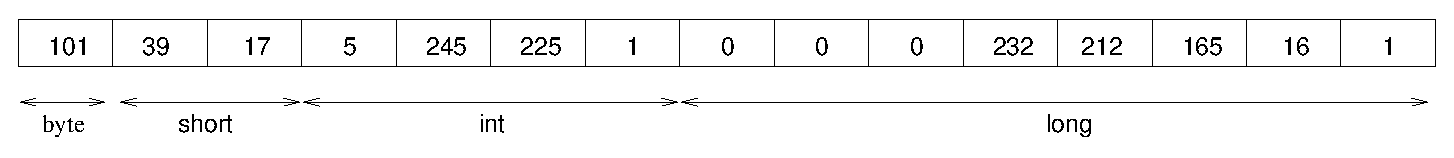
\includegraphics[width=\textwidth]{figures/messagecontents.eps}
%\end{center}
\jfigs{figures/messagecontents.eps}{\textwidth}
%
As you can see, the brute-force method requires the programmer to
do quite a bit of work: computing and naming
the offset and size of each value, and invoking the encoding routine
with the appropriate arguments. 
%
Fortunately, alternative ways to build messages are often available.
We discuss these next.

%%%%%%%%%%%%%%%%%%%%%%%%%%%%%%%%%%%%%%%%%%%%%%%%%%%%%%%%%%%%%%%%
% BEGIN C-SPECIFIC
%%%%%%%%%%%%%%%%%%%%%%%%%%%%%%%%%%%%%%%%%%%%%%%%%%%%%%%%%%%%%%%%

\subsection{Wrapping TCP Sockets in Streams}
\label{sect:streams}

A way of encoding multi-byte integers for transmission
over a stream (TCP) socket is to use the built-in
\type{FILE}-stream facilities---the same methods you use with
\var{stdin}, \var{stdout}, etc.  To access these facilities, you need
to associate one or more \type{FILE} streams with your socket
descriptor, via the \fcnsys{fdopen()} call.

\begin{inlinefcn}
\type{FILE *} \fcnsys{fdopen}(\type{int} \param{socketdes}, 
           \type{const char *}\param{mode});\\
\type{int} \fcnsys{fclose}(\type{FILE *} \param{stream});
\end{inlinefcn}

The \fcn{fdopen()} function ``wraps'' the socket in a stream and
returns the result (or NULL if an error occurs); it is as if you could
call \fcn{fopen()} on a network address.
This allows buffered I/O to be performed on the socket via operations like 
\fcn{fgets()}, \fcn{fputs()}, \fcn{fread()} and \fcn{fwrite()}.
\fcn{fclose()} closes the stream along with the underlying socket.
Note that \type{FILE}-streams are one-way abstractions: if you want to do
\emph{both\/} buffered input and output over a socket, you have to call
\fcn{fdopen()} once with mode ``r''
to get an input stream and again with mode ``w'' to get an
output stream. 

\begin{inlinefcn}
\type{size\_t} \fcnsys{fwrite}(\type{const void *}\param{ptr},
\type{size\_t} \param{size}, \type{size\_t} \param{nmemb}, \type{FILE
  *} \param{stream});\\
\type{size\_t} \fcnsys{fread}(\type{void *}\param{ptr},
\type{size\_t} \param{size}, \type{size\_t} \param{nmemb}, \type{FILE
  *}\param{stream});\\
\end{inlinefcn}

The \fcn{fwrite()} method copies \param{nmemb\/} objects, each of size
\param{size}, from the location \param{ptr} to the (output)
\param{stream}.  The \fcn{fread()} method goes the other direction,
reading the given number of objects of the given size from the given
stream and placing them sequentially in the location pointed to by
\param{ptr}.  Note that the sizes are given in units of
\fcn{sizeof}(\type{char}), while the return values of these methods
are the number of objects read/written, \emph{not\/} the number of
bytes.
In particular, \fcn{fread()} never reads \emph{part\/} of an object
from the stream, and similarly \fcn{fwrite()} never writes a partial
object.  If the underlying connection terminates, these methods will
return a short item count.

By giving different sizes to \fcn{fwrite}, we can output
our message to the stream sequentially.
Assume that the variables
\var{val8}, \var{val16}, etc. are declared and initialized as in
\file{BruteForceCoding.c}, and that the integer variable
\var{sock} is the descriptor of the connected TCP socket
over which we want to write our message.  Finally, assume that
\fcn{htonll()} is a function that converts 64-bit integers from host
to network byte order (see Exercise \ref{htonll}).
Then we can write our message to the socket one integer at a time:

% XXXXXX CODE NOT CHECKED
\begin{inlinecode}
  sock = socket(/*...*/);
  /* ... connect socket ...*/
  // wrap the socket in an output stream
  FILE *outstream = fdopen(sock,"w");
  // send message, converting each object to network byte order before sending
    if (fwrite(&var8, 1, sizeof(var8), outstream) < sizeof(var8)) ...
  var16 = htons(var16);
  if (fwrite(&var16, 1, sizeof(var16), outstream) <  sizeof(val16)) ...
  var32 = htonl(var32);
  if (fwrite(&var32, 1, sizeof(var32), outstream) < sizeof(val32)) ...
  var64 = htonll(var64);
  if (fwrite(&var64, 1, sizeof(var64), outstream) < sizeof(val64)) ...
  fflush(outstream); // be sure the values are written to the socket
  ...                // do other work...
  fclose(outstream); // closes the socket connection!
\end{inlinecode}

So much for the sending side.  How does the receiver recover the
transmitted values?  As you might expect, the receiving side takes the
analogous steps using \fcn{fread()}.  Suppose now the variable \var{csock}
contains the socket descriptor for a TCP connection, that the
received values are to be placed in the variables \var{rcv8},
\var{rcv16}, \var{rcv32}, and \var{rcv64} of the expected types, and
that \fcn{ntohll()} is a network-to-host byte order converter for
64-bit types.

% XXXX CODE NOT CHECKED
\begin{inlinecode}
  /* ... csock is connected ...*/
  // wrap the socket in an input stream
  FILE *instream = fdopen(csock,"r");
  // receive message, converting each received object to host byte order
  if (fread(&rcv8, 1, sizeof(var8), instream) < 1) ...
  if (fread(&rcv16, 1, sizeof(var16), instream) <  1) ...
  rcv16 = ntohs(rcv16); // convert to host order
  if (fread(&rcv32, 1, sizeof(rcv32), instream) < 1) ...
  rcv32 = ntohl(rcv32);
  if (fread(&rcv64, 1, sizeof(rcv64), instream) < 1) ...
  rcv64 = ntohll(rcv64);
  ...
  fclose(instream); // closes the socket connection!
\end{inlinecode}

Among the advantages of using buffered \type{FILE}-streams with sockets
is the ability to ``put back'' a byte after reading it from the
stream (via \fcn{ungetc()});
this can sometimes be useful when parsing messages.
\callout{We must emphasize, however, that \type{FILE}-streams can \emph{only\/} be used
with TCP sockets.}

\subsection{Structure Overlays: Alignment and Padding}
\label{sect:overlay}
The most common approach to constructing messages containing
binary data (i.e., multi-byte integers) involves overlaying a
C structure on a section of memory and assigning to the fields of the
structure directly.  This is possible because
the C language specification \emph{explicitly defines how structures
are laid out in memory by the compiler}.
It has this feature because it was designed for
implementing operating systems, where efficiency is a primary concern,
and it is often necessary to know precisely how data
structures are represented.
%
In combination with the facilities for byte order
conversion that we saw above, this makes it rather simple to construct
and parse messages made up of integers of particular sizes.  (There is
a significant caveat, however, that we will encounter shortly.)

Suppose for a moment that we are dealing with
three integer components of an address: the number on the street,
which ranges from 1 to about 12000, an apartment number that never exceeds
8000 (a non-apartment address uses an apartment number of $-1$),
and a postal code, which is a 5-digit number between 10000 and
99999.  The first two components can be represented using
16-bit integers; the third is too big for that, so we'll use a 32-bit
integer for it.
%
If we want to pass those quantities around inside a program, we could
declare a structure and pass around pointers to it:
%
\begin{inlinecode}
  struct addressInfo {
     uint16_t  streetAddress;
     int16_t  aptNumber;
     uint32_t   postalCode;
  } addrInfo;
\end{inlinecode}
%
Clearly such a structure is useful for passing data around in a
program, but can we use it pass information between programs over the
Internet?  The answer is yes.  The C specification says that this structure
will be laid out as follows in memory:

\jfigs{figures/addrstruct.eps}{0.6\textwidth}

To exchange information between programs, we can simply use the layout
of the structure as the message format, and take the contents directly
from the structure and send them over the network (after any needed
byte order conversions).
%
If the variable \var{addrInfo} declared above has been initialized to
contain the values we want to send,
and \var{sock} represents a connected socket as usual, we could send the
8-byte message using the following code:
%
\begin{inlinecode}
  // ... put values in addrInfo ...
  // convert to network byte order
  addrInfo.streetAddress = htons(addrInfo.streetAddress);
  addrInfo.aptNumber = htons(addrInfo.aptNumber);
  addrInfo.postalCode = htonl(addrInfo.postalCode);
  if (send(sock,&addrInfo,sizeof(addrInfo),0) < sizeof(addrInfo)) ...
\end{inlinecode}
%
On the receiving end, we can again use a buffered input stream (see
previous section) and \fcnsys{fread()} to handle getting
the right number of bytes into the structure.  (Otherwise we have to
use a loop because, as we saw earlier,
there is no guarantee the all the bytes of
the message will be returned in a single call to \fcn{recv()}).
Once that's done, all we have to do is take care of byte ordering:
\begin{inlinecode}
  struct addressInfo addrInfo;
  // ... sock is a connected socket descriptor ...
  FILE *instream = fdopen(sock,"r");
  if (fread(&addrInfo,1,sizeof(struct addressInfo),instream) < 1) {
    // ... handle error
  }
  // convert to host byte order
  addrInfo.streetAddress = ntohs(addrInfo.streetAddress);
  addrInfo.aptNumber = ntohs(addrInfo.aptNumber);
  addrInfo.postalCode = ntohl(addrInfo.postalCode);
  // use information from message...
\end{inlinecode}
%
%
Now, it would seem that we could construct our 15-byte
message using a declaration like the following:
%
\begin{inlinecode}
  struct integerMessage {
    uint8_t oneByte;
    uint16_t twoBytes;
    uint32_t fourBytes;
    uint64_t eightBytes;
  } 
\end{inlinecode}
%
Alas, this doesn't work, because the C language
rules for laying out data structures
include specific \emph{alignment\/} requirements, including that the
fields within a structure begin on certain boundaries based on their type.
The main points of the requirements can be summarized as follows:
\begin{itemize}
\item
Data structures are maximally aligned.  That is, the address of any
instance of a structure (including one in an array) will be divisible
by the size of its largest native integer field.
\item
Fields whose type is a multibyte integer type are aligned to their
size (in bytes).
Thus an \type{int32\_t} integer field's beginning address is always
divisible by four, and a \type{uint16\_t}
integer field's address is guaranteed to be divisible by two.
\end{itemize}
To enforce these constraints the compiler may add \emph{padding\/}
between the fields of a structure.  Because of this, the size of the
structure declared above is not 15, but \emph{16}.  To see why, let's
consider the constraints that apply.  First,
the whole structure must begin on an address divisible by 8.  The
\var{twoBytes} field must be at an even address, \var{fourBytes} must
be at an address divisible by four, and \var{eightBytes}' address must be
divisible by eight.  All of these constraints will be satisfied if a
single byte of padding is inserted between the \var{oneByte} field and
the \var{twoBytes} field, like this:
%
\jfigs{figures/intpaddedlayout.eps}{\textwidth}
%
The contents of bytes added by the compiler as padding are undefined.
Thus if the declaration above is used, and the receiver
is expecting the original unpadded layout, incorrect behavior is the
likely result.

The best solution is to avoid the need for padding by laying out
messages so that it is not needed.
Unfortunately (and somewhat surprisingly), that's not always possible.
In the case of our four-integer example, if we arranged the message
with fields in the opposite order:
\begin{inlinecode}
  struct backwardMessage {
    uint64_t eightBytes;
    uint32_t fourBytes;
    uint16_t twoBytes;
    uint8_t oneByte;
  } 
\end{inlinecode}
no padding would be required between the fields.
However, \fcn{sizeof(struct backwardMessage)}
would nevertheless return 16, not 15.
This is because one byte of padding would be required
\emph{between\/} instances of the
structure (in an array, for example), in order to satisfy the
first (maximal-alignment) constraint.
(The invariant that must be maintained is that in an array of
structures, the address of one element plus the \fcn{sizeof()} the
structure yields the address of the subsequent element.)
%
As a consequence, there is no way to specify
a structure containing any multi-byte integer for which \fcn{sizeof()}
returns an odd number.

If we can't eliminate compiler-required padding, we can, as a last
resort, include it in the message format specification.
For our example, the message format could be
defined with an \emph{explicit} padding byte after the first field:
\begin{inlinecode}
  struct integerMessage2 {
    uint8_t oneByte;
    uint8_t padding;   // Required for alignment
    uint16_t twoBytes;
    uint32_t fourBytes;
    uint64_t eightBytes;
  } 
\end{inlinecode}
This structure is laid out in memory \emph{exactly\/}
like the originally-declared \type{integerMessage}, except that
the contents of the padding byte can now be controlled and accessed by
the programmer. 
%
We'll see more examples of the use of structures to encode data in
Section~\ref{sect:binEncoding}.

\subsection{Strings and Text}

% XXXX not happy with this first paragraph yet.  Have to reach the
% poor student who knows NOTHING about what's going on in the machine.

Old-fashioned \emph{text\/}---strings of printable (displayable)
characters---is perhaps the most common way to represent information.
We've already seen examples of sending and receiving strings of text in
our echo client and server; you are probably also accustomed to having
programs you write generate text output.

Text is convenient because we deal with it all the time:
information is represented as strings of characters in books,
newspapers, and on computer displays.  Thus, once we know how to
encode text for transmission, it is straightforward to 
send most any other kind of data:
simply represent it as text, then encode the text.  You know how to
represent numbers and boolean values as strings of text---for example
\texttt{"123478962"}, \texttt{"6.02e23"}, \texttt{"true"},
\texttt{"false"}.  In this section we deal with the question of
encoding such strings as byte sequences.

% Here's some good stuff from the documentation for Charset.  It's
% probably beyond the scope of the book, but we should keep it in mind
% so we at least don't *misuse* any terminology.

%% The name of this class [i.e. Charset] is taken from the terms used
%% in RFC 2278. In that document a charset is defined as the
%% combination of a coded character set and a character-encoding scheme. 

%% A coded character set is a mapping between a set of abstract
%% characters and a set of integers. US-ASCII, ISO 8859-1, JIS X 0201,
%% and full Unicode, which is the same as ISO 10646-1, are examples of
%% coded character sets. 

%% A character-encoding scheme is a mapping between a coded character set
%% and a set of octet (eight-bit byte) sequences. UTF-8, UCS-2, UTF-16,
%% ISO 2022, and EUC are examples of character-encoding schemes. Encoding
%% schemes are often associated with a particular coded character set;
%% UTF-8, for example, is used only to encode Unicode. Some schemes,
%% however, are associated with multiple character sets; EUC, for
%% example, can be used to encode characters in a variety of Asian
%% character sets.

%% When a coded character set is used exclusively with a single
%% character-encoding scheme then the corresponding charset is usually
%% named for the character set; otherwise a charset is usually named for
%% the encoding scheme and, possibly, the locale of the character sets
%% that it supports. Hence US-ASCII is the name of the charset for
%% US-ASCII while EUC-JP is the name of the charset that encodes the JIS
%% X 0201, JIS X 0208, and JIS X 0212 character sets.

%% The native character encoding of the Java programming language is
%% UTF-16. A charset in the Java platform therefore defines a mapping
%% between sequences of sixteen-bit UTF-16 code units and sequences of
%% bytes.

% XXXXXX Is this too much?  Maybe we let the reviewers consider that
% question.. 

To that end, we first need to recognize that text is made up of
sequences of symbols, or \emph{characters}.  The C language includes
the primitive type \type{char} for representing characters, but does not
include a primitive type for strings.  Strings in C are
traditionally represented as arrays of \type{char}.
A \type{char} value in C is represented internally as an integer.
For example, the character \texttt{'a'}, that is, the symbol for the
letter `a', corresponds to the integer 97.  The character \texttt{'X'}
corresponds to 88, and the symbol \texttt{'!'} (exclamation mark)
corresponds to 33.

A mapping between a set of symbols and a set of integers is called a
\emph{coded character set}.  You may have heard of the
coded character set known as \emph{ASCII}---American Standard Code
for Information Interchange. ASCII maps the letters of the English
alphabet, digits, punctuation and some other special (non-printable)
symbols to integers between 0 and 127.
%
It has been used for data transmission since the 1960's, and is used
extensively in application protocols such as HTTP (the protocol used
for the world-wide web), even today.
%
The C language specifies a \emph{basic character set\/} that is a
subset of ASCII.  The importance of ASCII (and the C basic character
set) is that strings containing only characters from the basic set can
be encoded using one byte per character.  (Note that in 
our echo client and server from
Chapter~\ref{chap:tcp} the encoding was \emph{irrelevant}, because
the server did not interpret the received data at all.)

This is well and good if you speak and use a language (like English)
that can be represented using a small number of symbols.
However, consider that no more than 256 distinct symbols
can be encoded using one byte per symbol, and that
a large fraction of the world's people use languages
that have more than 256 symbols, and therefore have to be encoded using
more than eight bits per character.  Clearly the use of C
presents significant challenges for implementing code that is
``internationalizable.''  Mandarin is just one prominent example of a
language that requires thousands of symbols.

The C99 extensions standard defines a type \type{wchar\_t} (``wide
character'') to store characters from charsets that may use more than one
byte per symbol. In addition, various library functions are defined
that support conversion between byte sequences and arrays of
\type{wchar\_t}, in 
both directions.  (In fact, there is a wide character string version
of virtually every library function that operates on character
strings.)
To convert back and forth between wide strings and encoded char (byte)
sequences suitable for transmission over the network, we would use
the \fcnsys{wcstombs()} (``wide character
string to multi-byte string'') and \fcnsys{mbstowcs()} functions.
\begin{inlinecode}
  #include <stdlib.h>
  size_t wcstombs(char * restrict s, const wchar_t * restrict pwcs, size_t n);
  size_t mbstowcs(wchar_t * restrict pwcs, const char * restrict s, size_t n);
\end{inlinecode}
The first of these converts a sequence of wide characters from the
array pointed to by \param{pwcs} into a sequence of multi-byte
characters, and stores these multibyte characters into the array
pointed to by \param{s}, stopping if the next conversion would exceed
the limit of \param{n} total bytes or if a null character is stored.
The second does the same thing in the other direction.

As we have seen, for a coded character set that requires larger
integer values, there is more than one way to encode those
values for transmission over the network.
Thus, it is necessary that sender and receiver agree on how those integers
will be encoded as byte sequences.

As an example, consider a platform that uses 16-bit
integers internally to represent characters, and whose character set includes
ASCII as a subset---that is, the character `a' maps to 97, `X' to 88,
etc.  Using the wide character facilities we can declare a wide
character string:
\begin{inlinecode}
  wchar_t testString[] = "Test!";
\end{inlinecode}
The internal representation of this string uses six 16-bit integers
(including one for the terminating null (0) character).
However, there are several ways to encode those integers as a sequence
of 8-bit bytes:
\begin{itemize}
\item
Each character can be represented using two bytes, in big-endian
order.  In that case, the result of calling \fcn{wcstombs()} on
the wide string \type{``Test!''} would be the following sequence:
 0, 84, 0, 101, 0, 115, 0, 116, 0, 33.
\item
Alternatively, we could use two bytes in little-endian order,
which would give: 84, 0, 101, 0, 115, 0, 116, 0, 33, 0.
\item
We could use an encoding that maps symbols in the original
ASCII character set to single bytes (the same as their ASCII
encoding), and uses two bytes for symbols beyond ASCII.
If the high-order bit of a byte is set, it indicates the
next symbol is encoded with two bytes; otherwise it is an ASCII symbol
encoded with a single byte.  In this case the result after calling
\fcn{wcstombs()} would be the five-byte sequence 84, 101, 115, 116, 33. 
\end{itemize}
(Note that in these examples we did \emph{not\/} include the terminating
null (0) character.  The terminating null is an artifact of the
language, and not part of the string itself. It therefore should not
be transmitted with the string unless the protocol explicitly specifies that
method of marking the end of the string.

The bad news is that C99's wide character facilities
are \emph{not\/} designed to
give the programmer explicit control over the encoding scheme. Indeed,
they assume a single, fixed charset defined according to the
``locale'' of the platform.
Although the facilities support a variety of charsets, they do not
% XXXXX CHECK THIS
even provide the programmer any way to learn which charset or encoding
is in use.  In fact, the C99 standard states in several situations
that the effect of changing the locale's charset at runtime is undefined.
%
What this means is that if you want to implement a protocol using a
particular charset, you'll have to implement the encoding yourself.

% XXXXXXXXXXXXXXXXXXXXXXXXXXXXXXX
% The bottom line here is that even the C99 standard is vague about
% any particular character set.  The relevant concepts are there:
% converting between sequences of bytes and characters.  But does it
% even mention endian-ness of the integers in the mappings?
% Do the conversion functions handle this?
% XXX CHECK: LC_CTYPE category.


% XXXX REPLACE THIS WITH AN EXAMPLE?  DON'T KNOW HOW TO DO IT IN THIS LOCALE...

%% For example, if you call \texttt{"Test!".getBytes()}
%% on the platform on which this book was written, you get back the
%% encoding according to UTF-8:
%% %\begin{center}
%% %\includegraphics[width=2.5in]{figures/stringtest1.eps}
%% %\end{center}
%% \jfigs{figures/stringtest1.eps}{0.25\textwidth}
%% If you call \texttt{"Test!".getBytes("UTF-16BE")},
%% on the other hand, you get the following array:
%% %\begin{center}
%% %\includegraphics[width=\textwidth]{figures/stringtest2.eps}
%% %\end{center}
%% \jfigs{figures/stringtest2.eps}{0.7\textwidth}
%% In this case each value is encoded as a two-byte sequence, with the
%% high-order byte first.
%% From \texttt{"Test!".getBytes("IBM037")}, the result
%% is:
%% %\begin{center}
%% %\includegraphics[width=2.5in]{figures/stringtest3.eps}
%% %\end{center}
%% \jfigs{figures/stringtest3.eps}{0.25\textwidth}
%% The moral of the story is that \emph{sender and receiver must agree on
%% the representation for strings of text}.  The easiest way for them to
%% do that is to simply specify one of the standard charsets.

%% Note that the most significant bit of the 64-bit binary value of
%% 12345654321 is 0, so its signed (two's-complement) and unsigned
%% representations are the same.  More generally, the distinction between
%% $k$-bit signed and unsigned values is irrelevant for values that lie
%% in the range 0 through $2^{k-1}-1$.  Unfortunately, protocols often
%% use unsigned integers; Java's lack of unsigned integer types means
%% that some care is required in dealing with such values, especially in
%% decoding.  (See program \mono{ItemQuoteDecoderBin.java} in
%% Section~\ref{sect:binEncoding} for an example.)

%% As with strings, Java provides mechanisms to turn primitive integer
%% types into sequences of bytes and vice versa. In particular, streams
%% that support the \mono{DataOutput} interface have methods
%% \mono{writeShort()},
%% \mono{writeInt()},
%% and
%% \mono{writeLong()},
%% which allow those types to be written out directly.
%% These methods all write out the bytes of integer primitive
%% types in big-endian byte order using two's-complement representation.
%% Similarly, implementations of the \mono{DataInput}
%% interface have
%% methods
%% \mono{readInt()},
%% \mono{readShort()}, and so on.
%% The next section describes some ways to compose instances of these
%% classes.

\subsection{Bit-Diddling: Encoding Booleans}
\label{sect:bitdiddling}

\emph{Bitmaps} are a very compact way to encode boolean information,
which is often used in protocols.  The idea of a bitmap is that each
of the bits of an integer type can encode one boolean
value---typically with 0 representing false, and 1 representing true.
To be able to manipulate bitmaps, you need to know how to set and
clear individual bits using C's ``bit-diddling'' operations.  A
\emph{mask} is an integer value that has one or more specific bits set
to 1, and all others cleared (i.e., 0).  We'll deal here mainly with
32-bit maps and masks, but everything we say
applies to types of other sizes as well.

Let's number the bits of an integer's binary representation from 0 to 31,
where bit 0 is the least significant bit.  In general, the \type{uint32\_t}
value that has a 1 in bit position $i$, and a zero in all other bit
positions, is just $2^i$.  So bit 5 corresponds to the number 32,
bit 12 to 4096, etc.  Here are some example mask declarations:

\begin{inlinecode}
const int BIT5 = (1<<5);
const int BIT7 = 0x80;
const int BITS2AND3 = 12;   // 8+4
const int bitmap = 1234567;
\end{inlinecode}

\noindent To \emph{set\/} a particular bit in an \type{int} variable,
combine it with the mask for that bit using the bitwise-OR operation
(\verb+|+):

\begin{inlinecode}
bitmap |= BIT5;
// bit 5 is now one
\end{inlinecode}

\noindent To \emph{clear\/} a particular bit, bitwise-AND it with the
\emph{bitwise complement} of the mask for that bit (which has ones
everywhere except the particular bit, which is zero).  The bitwise-AND
operation in C is \verb+&+, while the bitwise-complement operator
is \verb+~+.

\begin{inlinecode}
bitmap &= ~BIT7;
// bit 7 is now zero
\end{inlinecode}

\noindent You can set and clear multiple bits at once by OR-ing
together the corresponding masks:

\begin{inlinecode}
// clear bits 2, 3 and 5
bitmap &= ~(BITS2AND3|BIT5);
\end{inlinecode}

\noindent To test whether a bit is set, compare the result of the
bitwise-AND of the mask and the value with zero:

\begin{inlinecode}
bool bit6Set = (bitmap & (1<<6)) != 0;
\end{inlinecode}

\section{Constructing, Framing and Parsing Messages}
\label{sect:parsing}%

We close this chapter with an example illustrating the
application of the foregoing techniques in implementing
a protocol specified by someone else.
The example is a simple ``voting'' protocol as shown in
\Fig{fig:VoteProto}.  Here a client sends a \emph{request\/} message
to the server; 
the message contains a candidate ID, which is an integer between 0 and
1000.  Two types of requests are supported. An \emph{inquiry\/} asks
the server how many votes have been cast for the given candidate.  The
server sends back a \emph{response\/} message containing the original candidate
ID and the vote total as of the time the request was received for
that candidate.  A \emph{voting\/} request actually casts a vote for
the indicated candidate.  The server again responds with a message
containing the candidate ID and the vote total (which now includes the
vote just cast).
The protocol runs over stream sockets using TCP.

\begin{figure}[htbp]
\begin{center}
%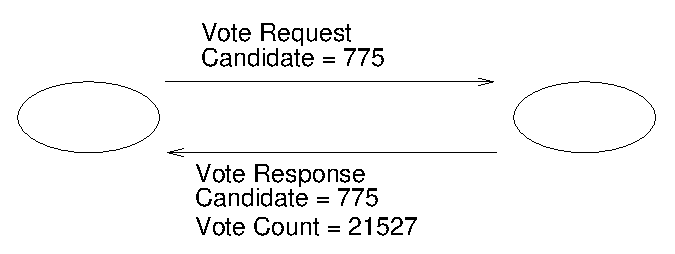
\includegraphics[width=4in]{figures/VoteProtocol.eps}
\jfigs{figures/VoteProtocol.eps}{0.6\textwidth}
\caption{Voting Protocol\label{fig:VoteProto}}
\end{center}
\end{figure}


Normally the ``wire format'' of the protocol
messages would be precisely defined as part of the protocol.
As we have seen, there are a number of ways we might encode it: we could
represent the information using strings of text, or as binary numbers.
In order to illustrate all the techniques described above, we will
specify several different versions of the ``wire format.''  This also
helps us to make a point about protocol implementation.

When implementing any protocol, it is good practice
to hide the details of the way messages are encoded from the main
program logic.
% 
We'll illustrate that here by using a generic structure in the main
programs to pass
information to/from functions that process messages sent/received over
the socket. 
%
This allows us to use the same client and server code with different
implementations of the ``wire format'' processing.
%
The \type{VoteInfo} structure, defined in \file{VoteProtocol.h},
contains everything needed to construct a message: the candidate ID number (an
integer), the count of votes for that candidate (a 64-bit integer),
a boolean indicating whether the message is an ``inquiry'' (inquiries do
not affect the vote count) and another boolean indicating whether the
message to be sent is a response sent from client to server (true), or
a request (false). 
%
Also defined in this file are constants for the largest allowable
candidate ID number and the maximum length of an encoded message on
the wire.  (The latter helps the programs to size their buffers.)
%
\begin{inlinecode}
struct VoteInfo {
  uint64_t count;   // invariant: !isResponse => count==0
  int candidate;    // invariant: 0 <= candidate <= MAX_CANDIDATE
  bool isInquiry;
  bool isResponse;
};

typedef struct VoteInfo VoteInfo;

enum {
    MAX_CANDIDATE = 1000,
    MAX_WIRE_SIZE = 500
};
\end{inlinecode}
Note that we have defined a single \type{VoteInfo} structure for
the information contained in \emph{both\/} request messages and
response messages. 
This, along with a proper control structure, allows re-use of the same
message-processing code for both client and server, and both
request and response.

The message-processing code is responsible for encoding the
information from a \type{VoteInfo} structure and transmitting it over a
stream socket, as well as for receiving data from a TCP socket,
parsing the incoming vote protocol message (if any), and filling in a
\type{VoteInfo} structure with the received information.

A clean design further decomposes the process into two parts.
The first is concerned with \emph{framing}, or marking the boundaries
of the message, so the receiver can find it in the stream.
The second is concerned with the actual encoding of the message,
whether it is represented using text or binary data.
%
Notice that these two parts can be independent of each other, and in a
well-designed protocol implementation they \emph{should\/} be separated.
In other words, we can specify the
mechanism for framing the message as a whole separately from the
encoding of its different fields.  And that is what we shall do.
%
Our job will be somewhat easier if we can use stream
processing functions, so we will have the client and server
wrap the connected socket in a \type{FILE} stream for input and
another for output. 

The interface to the framing code is defined as follows in \file{Framer.h}.
%
\begin{inlinecode}
int getNextMsg(FILE *in, uint8_t *buf, size_t bufSize);
void putMsg(uint8_t buf[], size_t msgSize, FILE *out);
\end{inlinecode}
%
The method \fcn{getNextMsg()} reads data from the given stream and places
it in the given buffer until it runs out of room or determines that it
has received a complete message.  It returns the number of bytes placed
in the buffer (all framing information is stripped).
The method \fcn{putMsg()} adds
framing information to the message contained in the given buffer, and
writes both message and framing information to the given stream.  Note that
neither of these methods needs to know \emph{anything\/} about the
message content.

The interface to the encoding and parsing code is defined in
\file{voteencoding.h} as follows:
%
\begin{inlinecode}
bool parse(uint8_t *inBuf, size_t mSize, VoteInfo *v);
size_t toWire(VoteInfo *v, uint8_t *outBuf, size_t bufSize);
\end{inlinecode}
%
The \fcn{toWire()} method takes a \type{VoteInfo} structure as input
and converts it to a sequence of bytes according to a particular
wire format encoding; it returns the size of the resulting byte
sequence.
%
The \fcn{parse()} method takes a byte sequence of a specified size and
parses it as a message according to the protocol, filling in the
\type{VoteInfo} with the information from the message.  It returns
\const{true} if the message was successfully parsed, and \const{false}
otherwise.

Given these interfaces to the framing and parsing code, we can now
describe the voting client and server programs that will use these
methods.
%
The client is straightforward: the candidate ID is given
as a command-line argument,  along with a flag indicating that the
transaction is an inquiry (by default it is a vote request).
Upon sending the request, the client waits for the response, and then
closes the connection when it is received.

\jcode{VoteClientTCP.c}{code/VoteClientTCP.c}{1}{1}

\begin{topcode}

\tlcitems{Access to library functions and constants}{1--14}

\tlcitems{Declarations and argument processing}{17--27}

\tlcitems{Get connected socket}{30--32}

\tlcitems{Wrap the socket in streams}{62--64}
We open the socket as a stream, once for writing and again for
reading, using \fcn{fdopen()}.

\tlcitems{Prepare and send request message}{67--83}
\begin{bottomcode}
%
\blcitems{Prepare a \type{VoteInfo} structure with the candidate
  ID}{67--71}
%
\blcitem{Encode into wire format}{74}
%
\blcitems{Print encoded message before framing}{82}
%
\blcitems{Add framing and send over the output stream}{85}
\end{bottomcode}
%
\tlcitems{Receive, parse, and process response}{85--98}
\begin{bottomcode}
\blcitem{Call \fcn{getNextMsg()}}{86}
The method handles all the messy details of receiving enough data through
the socket to make up the next message; like \fcn{recv()}, it may
block indefinitely.

\blcitem{Pass the result to be parsed}{87}

\blcitems{Process the response if it is correctly formed}{87--97}
Invalid responses are ignored.
\end{bottomcode}

\tlcitems{Close the streams}{101--103}

\end{topcode}

Turning now to the server, it needs a way to keep track of the vote counts
of all the candidates.  Because there are at most 1001 candidates, an
array of 64-bit integers will serve nicely.
The server prepares its socket and waits for incoming
connections like the other servers we have seen.  When a connection
arrives, it receives and processes messages over that connection until
the client closes it.
%
Note that, because of the very basic interface to the framing/parsing code, our
client and server are quite simple-minded when it comes to handling
errors in received messages; the server simply ignores any message
that is malformed and immediately closes the connection.

\jcode{VoteServerTCP.c}{code/VoteServerTCP.c}{1}{1}

\begin{topcode}
\tlcitems{Access to library functions and constants}{0--11}

\tlcitems{Local declarations}{13--16}

\tlcitems{Declarations and argument processing}{18-26}

\tlcitem{Set up to receive}{28}

\tlcitems{Repeatedly accept and handle clients}{31--79}

\begin{bottomcode}
\blcitem{Reset the data area}{37}

\blcitems{Wait for connection}{40}

\blcitems{Print client info}{45--51}

\blcitems{Wrap the socket in streams}{53--56}

\blcitems{Receive and process messages until connection closes}{60--77}
Note that the server uses the same code as the client to parse,
frame, and encode messages.
\end{bottomcode}

\tlcitem{Array to store vote counts}{81}

\tlcitems{Request handler}{83--93}
\end{topcode}

\subsection{Framing}
\label{sect:framing}

Application protocols typically deal
with discrete messages, which are viewed as collections of fields.
\emph{Framing} refers to the general problem of enabling the receiver to
locate the boundaries of a message (or part of one).
Whether information is
encoded as text, as multibyte binary numbers, or as some combination
of the two, the application protocol must specify how the receiver of
a message can determine when it has received all of the message.

Of course, if a complete message is sent as the payload
of a UDP datagram, the problem is trivial:
every send/receive operation on a datagram socket involves a single
message, so the receiver knows exactly where that message ends.
For messages sent over TCP sockets, however, the situation can be more
complicated, because TCP has no notion of message boundaries.
If the fields in a message all have fixed sizes and the message is
made up of a fixed number of fields, then
the size of the message is known in advance and the receiver
can simply read the expected number of bytes into a buffer.
(This  technique was used in \file{TCPEchoClient.java}, where
we knew the number of bytes to expect from the server.)
However, when the message can vary in length---for example, if it
contains some variable-length arbitrary text strings---we do
not know beforehand how many bytes to read.

If a receiver tries to receive more bytes from a socket
than were in the message, one of two things can happen.  If no other
message is in the channel, the receiver will block,
and be prevented from processing the message; if the sender is also
blocked waiting for a reply, the result will be \emph{deadlock}: each
side of the connection waiting for the other to send more information.
% XXX could put a footnote here about nonblocking not being the answer...
On the other hand, if another message is in the channel,
the receiver may read some or all of it as part of the first message,
leading to other kinds of errors.
Therefore framing is an important consideration when using TCP sockets.

Note that some of the same considerations apply to finding the
boundaries of the individual \emph{fields\/} of the message:
the receiver needs to know where one ends and another begins.
Thus, pretty much everything we say here about framing messages
also applies to fields.
However, as was pointed out above, the cleanest code results if we
deal with the problem of locating the end of the message separately
from that of parsing it into fields.

Two general techniques enable a receiver to
unambiguously find the end of the message:
%
\begin{itemize}
\item \emph{Delimiter-based}: The end of the message
is indicated by a \emph{unique marker}, an explicit byte (or sequence
of bytes) that the sender transmits immediately following the data.
%The marker must be known not to occur in the data.
\item \emph{Explicit length}: The variable-length field or message
is preceded by a  \emph{length\/} field
that tells how many bytes it contains.  The length field is generally
of a fixed size; this limits the maximum size message that can be framed.
\end{itemize}
%
A special case of the delimiter-based method can be used for
the last message sent on a TCP
connection: the sender simply closes the sending side of the
connection (using \fcn{shutdownOutput}
or \fcn{close})
after sending the message.
After the receiver reads the last byte of the message, it
receives an end-of-stream indication (i.e., \fcn{read}
and thus can tell that it has reached the end of the message.
% XXXXXX The foregoing may conflict with the actual implementation of
% the framing protocol below, which does NOT accept EOS as a delimiter.

The delimiter-based approach is often used with messages encoded as text:
A particular character 
or sequence of characters is defined to mark the end of the message.
The receiver simply scans the input (as characters) looking for the delimiter
sequence; it returns the character string preceding the delimiter.
The drawback is that \emph{the message itself must not contain the delimiter};
otherwise the receiver will find the end of the message prematurely.
With a delimiter-based framing method, someone has to be
responsible for ensuring that this precondition is satisfied.
%
Fortunately, so-called \emph{stuffing\/} techniques allow delimiters
that occur naturally in the message to be modified so the receiver
will not recognize them as such.  The sending side performs a
transformation on delimiters that occur in the text;
the receiver, as it scans for the delimiter, it
also recognizes the transformed delimiters, and restores them so the
output message matches the original.
The downside of such techniques is that \emph{both\/}
sender and receiver have to scan every byte of the message.

The length-based approach is simpler, but requires a known upper bound
on the size of the message.  The sender first determines the length of
the message, encodes it as an integer, and prefixes the result to the
message.  The upper bound on the message length determines the number
of bytes required to encode the length: one byte if messages always
contain fewer than 256 bytes, two bytes if they are always shorter
than 65536 bytes, and so on.

The module \file{DelimFramer.c} implements delimiter-based framing
using the ``newline'' character (\verb+"\n"+, byte value 10) as the
delimiter.  Our \fcn{putMsg()} method does
\emph{not\/} do stuffing, but simply fails (catastrophically) if the
% XXXXX CHECK IT
byte sequence to be framed already contains the delimiter.
%
The \fcn{getNextMsg()} method scans the stream, copying each byte
into the buffer until it reads the delimiter or runs out of space.
It returns the number of bytes placed in the buffer.
If the message is truncated, i.e. the method returns a full buffer
without encountering a delimiter, the returned count is negative.
If some bytes of a message are
accumulated and the stream ends without finding a delimiter,
it is considered an error and a negative value is returned (i.e., this
protocol does \emph{not\/} accept end-of-stream as a delimiter.
Thus, an empty but correctly-framed message (length zero is returned)
can be distinguished from the stream ending.

\jcode{DelimFramer.c}{code/DelimFramer.c}{1}{1}

% XXXX LINES PROBABLY OFF
\begin{topcode}

\tlcitems{Declare constant delimiter value.}{5--7}

\tlcitems{input method: \fcn{getNextMsg()}}{17--32}

\begin{bottomcode}

\blcitem{initialize byte count}{18}
Check that the given message does not contain the
delimiter; if so, throw an exception.

\blcitems{iterate until buffer is full or EOF}{20--31}
We get the next byte from the input stream, compare it to EOF, then
the delimiter.  On EOF we abort if an
incomplete message is in the buffer, else return -1. On delimiter we
break out of the loop.

\blcitem{return the count of bytes transferred to buffer}{32}
\end{bottomcode}

\tlcitems{Output method: \fcn{putMsg}}{38--48}

\begin{bottomcode}

\blcitem{Scan the input message looking for the delimiter}{41--43}
If we find it, (we rather unhelpfully) kill the program.

\blcitem{Write message to output stream}{44}

\blcitem{Write delimiter byte to output stream}{46}

\blcitem{Flush the output stream}{47}
This ensures that the message is sent over the underlying socket.
\end{bottomcode}

\end{topcode}

While our implementation makes it fairly easy to change the single
character used as a delimiter,
some protocols make use of multiple-character delimiters.
The HTTP protocol, which is used in the world-wide web, uses
text-encoded messages delimited by the four-character sequence
\verb+\r\n\r\n+.
Extending the delimiter-based framing module to support multicharacter
delimiters and to handle stuffing are left as exercises.

The module \file{LengthFramer.c} implements the framing interface
using length-based framing.  It works for messages up to 65,535
($2^{16}-1$) bytes in length.  The \fcn{putMsg()} method
determines the length of the given message and writes it to the output
stream as a two-byte, big-endian integer, followed by the complete
message.  On the receiving side, the \fcnsys{fread()} method is used
to read the length as an integer; after converting it to host byte
order, that many bytes are read from the channel.
Note that, with this framing method, the
sender does not have to inspect the content of the message being
framed; it needs only to check that the message does not exceed the
length limit.

\jcode{LengthFramer.c}{code/LengthFramer.c}{1}{1}

\begin{topcode}

\tlcitems{input method: \fcn{getNextMsg()}}{11--24}
\begin{bottomcode}
%
\blcitem{Read the prefix length}{14}
The \fcn{fread()} method reads two bytes into the unsigned 16-bit
integer \var{mSize}.
%
\blcitem{Convert to host byte order}{16}

\blcitems{Truncate message if necessary}{18--21}
If the indicated size is bigger than the buffer provided by the
caller, we truncate the message so it will fit, and remember so 
we can indicate via the return value that we did so.
(Note that in this case, the remainder of the message is left in the
channel. [XXX FIX THIS?])

\blcitem{Read the message}{19}
\blcitems{Return the size}{20--23}
\end{bottomcode}

\tlcitems{Output method: \fcn{putMsg}}{29--38}
\begin{bottomcode}
\blcitems{Verify input length}{30--31}
Because we use a two-byte unsigned length field, the length cannot exceed
65535 (the value of \const{uint16\_max}).
%
\blcitem{Convert length to network byte order}{32}
\blcitems{Output length}{33--34}
\blcitems{Output message}{35--36}
\blcitem{Flush to ensure the message is sent}{37}
\end{bottomcode}
\end{topcode}


\subsection{Text-Based Message Encoding}
\label{sect:textEncoding}%

Now we turn to the representation of voting messages as text.
Because we only have to represent numbers and a couple of
indicators, we can use the basic C charset US-ASCII.
The message consists of text fields separated by one or more
occurrences of the ASCII space character (decimal value 32).
The message begins with a so-called ``magic string''---a
sequence of ASCII characters that allows a recipient to quickly recognize
the message as a Voting protocol message, as opposed to random garbage
that happened to arrive over the network.  The Vote/Inquiry boolean is
encoded with the character `v' for a vote or `i' for an inquiry.  The
message's status as a response is indicated by the presence of the
character `R'.  Then comes the candidate ID, followed by the vote
count, both encoded as strings of decimal digits.
The module \file{VoteEncodingText.c} implements
this text-based encoding.

\jcode{VoteEncodingText.c}{code/VoteEncodingText.c}{1}{1}

The \fcn{toWire} method uses \fcnsys{snprintf()} to construct a string
containing all the fields of the message, separated by whitespace.  It
fails only if the caller provides an insufficient amount of space to
hold the string.

The \fcn{parse()} method uses the \fcnsys{strtok()} method to
break the received message into tokens (fields).  The \fcn{strtok()}
library function takes a pointer to a character array and a string
containing characters to be interpreted as delimiters.
The first time it is called, it returns the
largest initial substring consisting entirely of characters not in the
delimiter string; the trailing delimiter of that string is replaced by
a null byte.  On subsequent calls with a NULL first argument, tokens
are taken left to right from the original string until there are no
more tokens, at which point NULL is returned.

\fcn{parse()} first looks for the ``Magic'' string; if
it is not the first thing in the message, it simply fails and returns
\const{false}.
%
\textbf{Note well:}
This illustrates a very important point about implementing protocols:
\emph{never assume anything about any input from the network}.  Your
program must always be prepared for any possible inputs, and handle
them gracefully.  In this case, the \fcn{parse()} method simply ignores
the rest of the message and returns \const{false} if some expected part is not
present or improperly formatted.\footnote{This also illustrates a key
  reason why it is best to do framing 
  before parsing: recovery from a parse error when a message has only
  been partially received is much more complex, because the receiver
  has to get ``back in sync'' with the sender.%
}
%
Otherwise, \fcn{parse()} gets
the fields token by token, using the library functions \fcnsys{atoi()}
and \fcnsys{strtoll} to convert tokens into integers.

\subsection{Binary Message Encoding}
\label{sect:binEncoding}

Next we present a different way to encode the Voting protocol message.
In contrast with the text-based format, the binary format uses
fixed-size messages.  Each message begins with a one-byte field that
contains the ``magic'' value 010101 in its high-order six bits.  As
with the text format, this
little bit of redundancy provides the receiver with a small degree of
assurance that it is receiving a proper voting message.  The two
low-order bits of the first byte encode the two booleans; note the use
of the bitwise-or operations shown above to set the flags.  The second
byte of the message always contains zeros (it is effectively padding)
and the third and fourth
bytes contain the candidateID.  The final eight bytes of a response
message (only) contain the vote count.

\jcode{VoteEncodingBin.c}{code/VoteEncodingBin.c}{1}{1}

The \fcn{parse()} method's job is especially simple in this
version---it simply copies the values from the message into the
\type{VoteInfo} structure, converting byte order along the way.

\subsection{Putting It All Together}

To get a working vote server, we simply compile together
\file{VoteServerTCP.c}, one of the two framing modules, one of the two
encoding modules, and the auxiliary modules \file{DieWithMessage.c},
\file{SetUpServer.c}, % XXX
and \file{Utility.c}.  For example:

\begin{shell}
\prompt \typed{gcc -o vs VoteServerTCP.c DelimFramer.c
  VoteEncodingBin.c} $\backslash$ \\
\hspace{1em} \typed{DieWithMessage.c SetUpServer.c Utility.c}\\
\prompt \typed{gcc -o vc VoteClientTCP.c DelimFramer.c
  VoteEncodingBin.c} $\backslash$ \\
\hspace{1em} \typed{DieWithMessage.c SetUpServer.c Utility.c}\\
\prompt
\end{shell}

All four possible combinations of framing method and encoding will
work---provided the client and server both use the same combination!

\section{Wrapping Up}

We have seen how primitive types can be represented as sequences of
bytes for transmission ``on the wire''.  We have also considered some
of the subtleties of encoding text strings, and some basic methods of
framing and parsing messages.  We saw examples of both text-oriented
and binary-encoded protocols.

It is probably worth reiterating something we said in the Preface:
this chapter will by no means make you an expert!  That takes a great
deal of experience. But the code from this chapter can be used as a
starting point for further explorations.

\begin{exercises}
\item
If the underlying hardware platform is little-endian, and
``network byte order'' is big-endian, is there any reason for
the implementations of \fcn{htonl()} and \fcn{ntohl()} to be different?

\item
\label{htonll}
Write the function \type{uint64\_t} \fcn{htonll(\type{uint64\_t}
\param{val})}, which converts a 64-bit integer from little-endian to
big-endian byte order.

\item
Write the little-endian analogs of the method given in
\file{BruteForceEncoding.c}, i.e., \fcn{encodeLittleEndian()} and
\fcn{decodeLittleEndian()}. 

\item
Write methods \fcn{encodeBigEndianSigned()} and
\fcn{decodeBigEndianSigned()}, which return signed values. (The
input buffers are still unsigned types. Hint: use explicit type-casting.) 

\item
The \fcn{encodeIntBigEndian()} method in
\file{BruteForceEncoding.c} only works if several preconditions
such as $0 \leq size \leq 8$ are satisfied.
Modify the method to test for these
preconditions and return an error indication of some sort if any are
violated.  What are the advantages and disadvantages of having the
program check the preconditions, versus relying on the caller to
establish them?

\item Assuming all byte values are equally likely, what is the
probability that a message consisting of random bits will pass the
``magic test'' in the binary encoding of the Voting protocol?
Suppose an ASCII-encoded text
message is sent to a program expecting a binary-encoded voteMsg. Which
characters would enable the message to pass the ``magic test'' if they
are the first in the message?

\item Suppose we use \file{DelimFraming.c} and
  \file{VoteEncodingBin.c} in building the Voting Client.  Describe
circumstances in which the client fails to send a message.

\item
Extend the delimiter-based framing implementation to perform ``byte stuffing'',
so that messages that contain the delimiter can be transmitted without
the caller of \fcn{putMsg()} having to worry about it.
That is, the framing module transparently
handles messages that contain the delimiter.
(See any decent networking text for the algorithm.)

\item
Extend the delimiter-based framing implementation to handle
arbitrary multiple-byte delimiters.  Be sure your implementation is
efficient.  (\textbf{Note}: this problem is \emph{not\/} trivial!  A naive
approach will run very inefficiently in the worst case.)

\item
Both \fcn{getNextMsg()} implementations truncate the received message
if the caller fails to provide a big enough message.  Consider the
behavior on the next call to \fcn{getNextMsg()} after this happens,
for both implementations.  Is the behavior the same in both cases?
If not, suggest modifications so that both implementations behave the
same way in all cases.
\end{exercises}
